\frame{
\frametitle{Docker Storage}
Every piece of data in Docker is a layer.
\vspace{0.4cm}
Layers can be (are) resued when possible.
\vspace{0.4cm}
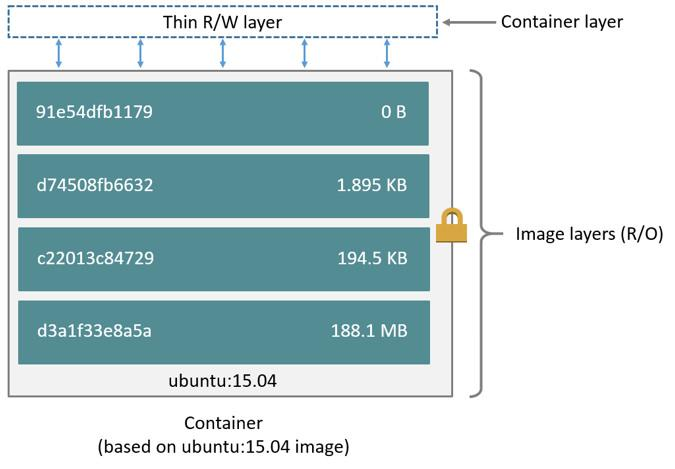
\includegraphics[width=0.50\columnwidth]{./Figure/docker-064-046}
}

\frame{
\frametitle{Docker Storage}
\framesubtitle{Layers}
Layers are a sort of snapshots of a filesystem
\vspace{0.4cm}
Usually are in readonly mode
\vspace{0.4cm}
To every new container a \it{Thin} r/w layer is created. In this layer the container can store its own data.
}

\begin{frame}[fragile]
\frametitle{Docker Storage}
\framesubtitle{Layers}
\begin{columns}
\begin{column}{.65\textwidth}
\begin{lstlisting}
FROM ubuntu:15.04
COPY ./app
RUN make /app
CMD python /app/app.py
\end{lstlisting}
\end{column}
\begin{column}{.35\textwidth}
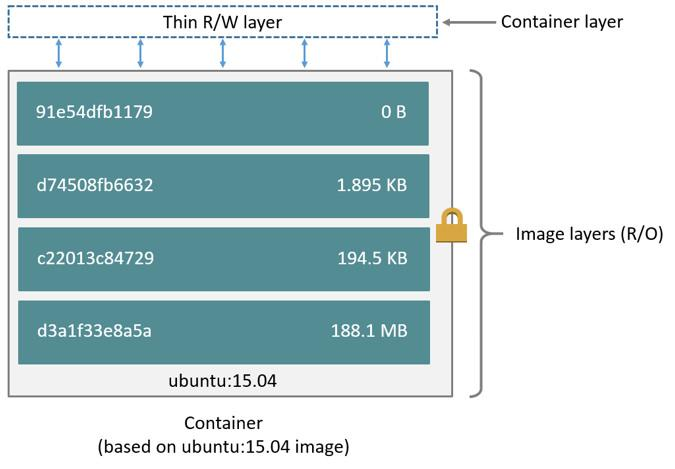
\includegraphics[width=1\columnwidth]{./Figure/docker-064-046}
\end{column}
\end{columns}
\end{frame}

\begin{frame}[fragile]
\frametitle{Docker Storage}
\framesubtitle{Pull and Storage}
\begin{lstlisting}
$ docker pull ubuntu:15.04

15.04: Pulling from library/ubuntu
1ba8ac955b97: Pull complete
f157c4e5ede7: Pull complete
0b7e98f84c4c: Pull complete
a3ed95caeb02: Pull complete
Digest: sha256:5e279a9df07990286cce22e1b0f5b049062
	9ca6d187698746ae5e28e604a640e
Status: Downloaded newer image for ubuntu:15.04
\end{lstlisting}
\end{frame}

\begin{frame}[fragile]
\frametitle{Docker Storage}
\framesubtitle{Pull and Storage}
\begin{lstlisting}
$ docker pull ubuntu:18.04
18.04: Pulling from library/ubuntu
124c757242f8: Pull complete
9d866f8bde2a: Pull complete
fa3f2f277e67: Pull complete
398d32b153e8: Pull complete
afde35469481: Pull complete
Digest: sha256:de774a3145f7ca4f0bd144c7d4ffb2931e0
	6634f11529653b23eba85aef8e378
Status: Downloaded newer image for ubuntu:18.04
\end{lstlisting}
\end{frame}


\begin{frame}[fragile]
\frametitle{Docker Storage}
\framesubtitle{Pull and Storage}
\begin{lstlisting}
$ docker images -f reference='ubuntu'

REPOSITORY   TAG     IMAGE ID      CREATED      SIZE
ubuntu       18.04   cd6d8154f1e1  2 weeks ago  84.1MB
ubuntu       16.04   2dc7f0e4fc33  2 years ago  122MB
ubuntu       14.04   54060fb55e83  3 years ago  188MB
\end{lstlisting}
\end{frame}

\begin{frame}[fragile]
\frametitle{Docker Storage}
\framesubtitle{Pull and Storage}
\begin{lstlisting}
$ sudo find /var/lib/docker -name cd6d81*

/var/lib/docker/image/aufs/imagedb/content/sha256/
	cd6d8154f1e16e38493c3c2798977c5e142be5e5d41403
	ca89883840c6d51762

\end{lstlisting}
\end{frame}

\begin{frame}
\frametitle{Docker Storage}
\framesubtitle{Drivers}
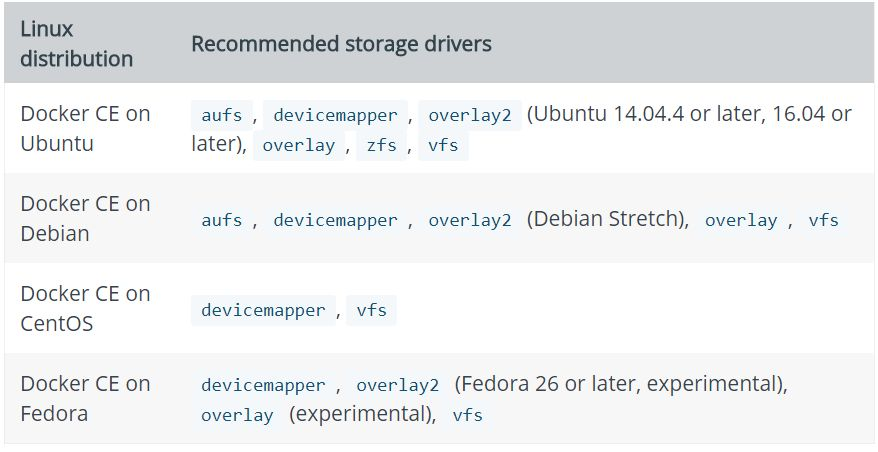
\includegraphics[width=1.0\columnwidth]{./Figure/docker-070-052}
\end{frame}

\begin{frame}
\frametitle{Docker Storage}
\framesubtitle{Drivers}
\begin{itemize}
\item aufs, overlay, overlay2: work at file level, memory efficient but layers can grow and become inefficient with high I/O
\item devicemapper,btrfs, zfs: block-level storage, works with write-heavy I/O
\item btrfs, zfs: require a lot of memory
\item zfs: is a good choice for high-density workloads such as PaaS
\item overlay: works better with many layers and small files compared to overlay2
\end{itemize}
\end{frame}


\begin{frame}
\frametitle{Docker Storage}
\framesubtitle{Drivers}

How to choose the driver:
\begin{itemize}
\item Perform tests based on your hardware with your sysadmin
\item Check the stability of the driver and decide your stability policy
\item If you have an expertise in house use it
\item Some drivers works best on some Linux distro
\item Perform tests on real workloads
\end{itemize}
\end{frame}

\begin{frame}
\frametitle{Docker Storage}
\framesubtitle{Drivers}
\it{!!! WARING !!!}
\vspace{0.4cm}
You can not mix drivers
\vspace{0.4cm}
Each driver has its set of images and containers
\vspace{0.4cm}
Migration is not possible
\end{frame}


\begin{frame}
\frametitle{Docker Storage}
\framesubtitle{Layers}
Layers are a sort of snapshots of a filesystem
\vspace{0.4cm}
Usually are in readonly mode
\vspace{0.4cm}
To every new container a \it{Thin} r/w layer is created. In this layer the container can store its own data.
\end{frame}

\begin{frame}
\frametitle{Docker Storage}
\framesubtitle{Thin layers}
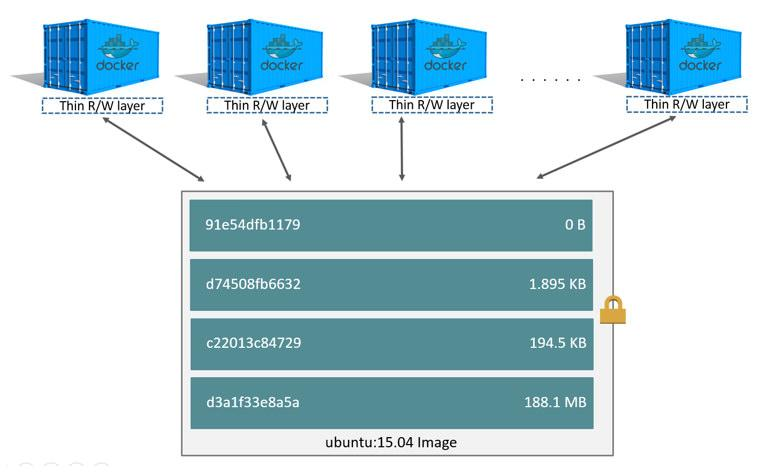
\includegraphics[width=0.5\columnwidth]{./Figure/docker-065-047}
\end{frame}


\begin{frame}
\frametitle{Docker Storage}
\framesubtitle{Thin layers and Data}
A writable container layer is created every time a container starts and it is where data are stored.
\vspace{0.4cm}
When a container is not running:
\begin{itemize}
\item Data does not persist
\item Sharing data with other container is very very ... very complicated
\item Your host machine own the writable layer, moving the layer is not that simple
\item Not the best option for high I/O, layers can be asynchronous 
\end{itemize}
\end{frame}

\begin{frame}[fragile]
\frametitle{Docker Storage}
\framesubtitle{Thin layers}
\begin{lstlisting}
$ docker run -dit --name my_container_1
           acme/my-final-image:1.0 bash

c36785c423ec7e0422b2af7364a7ba4da6146cbba7981a0951
	fcc3fa0430c409


$ docker run -dit --name my_container_2 
           acme/my-final-image:1.0 bash
		   
dcad7101795e4206e637d9358a818e5c32e13b349e62b00bf0
	5cd5a4343ea513

...
\end{lstlisting}
\end{frame}

\begin{frame}[fragile]
\frametitle{Docker Storage}
\framesubtitle{Thin layers, where are }
\begin{lstlisting}
$ sudo du -shL /var/lib/docker/containers/*
32K /var/lib/docker/containers/1a174fc216cccf18ec7
	d4fe14e008e30130b11ede0f0f94a87982e310cf2e765
32K /var/lib/docker/containers/1e7264576d78a3134fb
	af7829bc24b1d96017cf2bc046b7cd8b08b5775c33d0c
32K /var/lib/docker/containers/38fa94212a419a082e6
	a6b87a8e2ec4a44dd327d7069b85892a707e3fc818544
32K /var/lib/docker/containers/c36785c423ec7e0422b
	2af7364a7ba4da6146cbba7981a0951fcc3fa0430c409
32K /var/lib/docker/containers/dcad7101795e4206e63
	7d9358a818e5c32e13b349e62b00bf05cd5a4343ea513 
\end{lstlisting}
\end{frame}

\begin{frame}[fragile]
\frametitle{Docker Storage}
\framesubtitle{Container and Size}
Running a plain Ubuntu 18.04
\vspace{0.4cm}
\begin{lstlisting}
$ docker run ubuntu -it ubuntu:18.04 bash
\end{lstlisting}
\vspace{0.4cm}
\it{Note} detach from the container using \lstinline!Ctrl-P! + \lstinline!Ctrl-Q!
\end{frame}

\begin{frame}[fragile]
\frametitle{Docker Storage}
\framesubtitle{Container and Size}
\begin{lstlisting}
$ docker ps -s


| CONTAINER ID | IMAGE        | SIZE                |

| 0e7438744a0a | ubuntu:18.04 | 0B (virtual 84.1MB) |
\end{lstlisting}
\end{frame}

\begin{frame}[fragile]
\frametitle{Docker Storage}
\framesubtitle{Container and Size}
Updating the \lstinline!apt! database
\vspace{0.4cm}
\begin{lstlisting}
$ docker attach 0e74

$ apt update


| CONTAINER ID | IMAGE        | SIZE                   |

| 0e7438744a0a | ubuntu:18.04 | 41.7MB (virtual 126MB) |
\end{lstlisting}
\end{frame}

\begin{frame}[fragile]
\frametitle{Docker Storage}
\framesubtitle{Container and Size}
Upgrading the \lstinline!apt! database
\vspace{0.4cm}
\begin{lstlisting}
$ apt upgrade


| CONTAINER ID | IMAGE        | SIZE                   |

| 0e7438744a0a | ubuntu:18.04 | 42.6MB (virtual 127MB) |
\end{lstlisting}
\end{frame}

\begin{frame}[fragile]
\frametitle{Docker Storage}
\framesubtitle{Container and Size}
Installing \lstinline!wget!
\vspace{0.4cm}
\begin{lstlisting}
$ apt install wget


| CONTAINER ID | IMAGE        | SIZE                   |

| 0e7438744a0a | ubuntu:18.04 | 49.1MB (virtual 133MB) |
\end{lstlisting}
\end{frame}

